\documentclass[
  bibliography=totoc,     % Literatur im Inhaltsverzeichnis
  captions=tableheading,  % Tabellenüberschriften
  titlepage=firstiscover, % Titelseite ist Deckblatt
]{scrartcl}

% Paket float verbessern
\usepackage{scrhack}

% Besser integriert in das KOMA-Skript-Bundle
\usepackage{scrlayer-scrpage}

% Warnung, falls nochmal kompiliert werden muss
\usepackage[aux]{rerunfilecheck}

% unverzichtbare Mathe-Befehle
\usepackage{amsmath}
% viele Mathe-Symbole
\usepackage{amssymb}
% Erweiterungen für amsmath
\usepackage{mathtools}

% Fonteinstellungen
\usepackage{fontspec}
% Latin Modern Fonts werden automatisch geladen
% Alternativ zum Beispiel:
%\setromanfont{Libertinus Serif}
%\setsansfont{Libertinus Sans}
%\setmonofont{Libertinus Mono}

% Wenn man andere Schriftarten gesetzt hat,
% sollte man das Seiten-Layout neu berechnen lassen
\recalctypearea{}

% deutsche Spracheinstellungen
\usepackage[ngerman]{babel}


\usepackage[
  math-style=ISO,    % ┐
  bold-style=ISO,    % │
  sans-style=italic, % │ ISO-Standard folgen
  nabla=upright,     % │
  partial=upright,   % ┘
  warnings-off={           % ┐
    mathtools-colon,       % │ unnötige Warnungen ausschalten
    mathtools-overbracket, % │
  },                       % ┘
]{unicode-math}

% traditionelle Fonts für Mathematik
\setmathfont{Latin Modern Math}
% Alternativ zum Beispiel:
%\setmathfont{Libertinus Math}

\setmathfont{XITS Math}[range={scr, bfscr}]
\setmathfont{XITS Math}[range={cal, bfcal}, StylisticSet=1]

% Zahlen und Einheiten
\usepackage[
  locale=DE,                   % deutsche Einstellungen
  separate-uncertainty=true,   % immer Unsicherheit mit \pm
  per-mode=symbol-or-fraction, % / in inline math, fraction in display math
]{siunitx}

% chemische Formeln
\usepackage[
  version=4,
  math-greek=default, % ┐ mit unicode-math zusammenarbeiten
  text-greek=default, % ┘
]{mhchem}

% richtige Anführungszeichen
\usepackage[autostyle]{csquotes}

% schöne Brüche im Text
\usepackage{xfrac}

% Standardplatzierung für Floats einstellen
\usepackage{float}
\floatplacement{figure}{htbp}
\floatplacement{table}{htbp}

% Floats innerhalb einer Section halten
\usepackage[
  section, % Floats innerhalb der Section halten
  below,   % unterhalb der Section aber auf der selben Seite ist ok
]{placeins}

% Seite drehen für breite Tabellen: landscape Umgebung
\usepackage{pdflscape}

% Captions schöner machen.
\usepackage[
  labelfont=bf,        % Tabelle x: Abbildung y: ist jetzt fett
  font=small,          % Schrift etwas kleiner als Dokument
  width=0.9\textwidth, % maximale Breite einer Caption schmaler
]{caption}
% subfigure, subtable, subref
\usepackage{subcaption}

% Grafiken können eingebunden werden
\usepackage{graphicx}

% schöne Tabellen
\usepackage{booktabs}

% Verbesserungen am Schriftbild
\usepackage{microtype}




% Hyperlinks im Dokument
\usepackage[
  german,
  unicode,        % Unicode in PDF-Attributen erlauben
  pdfusetitle,    % Titel, Autoren und Datum als PDF-Attribute
  pdfcreator={},  % ┐ PDF-Attribute säubern
  pdfproducer={}, % ┘
]{hyperref}
% erweiterte Bookmarks im PDF
%\usepackage{bookmark}

% Trennung von Wörtern mit Strichen
\usepackage[shortcuts]{extdash}
% Kopfnoten
\ihead{\href{https://www.tu-dortmund.de/}{
\includegraphics[height=25pt]{TUlogo.png}}}  % links
\ohead{\href{https://physik.tu-dortmund.de/}{
\includegraphics[height=25pt]{FAKlogo.png}}}  % rechts
\chead{\href{mailto:jan.gaschina@tu-dortmund.de}{Jan Gaschina}}	 % center
\KOMAoptions{headsepline = 0.5pt:text}  % Dicke:Breite

%\KOMAoptions{pagenumber = off}

% Fußnoten
 \ifoot{}  % links
 \cfoot[\pagemark]{Seite \pagemark}  % center, 
\ofoot[]{}  % rechts
\KOMAoptions{footsepline = 0.5pt:text}  % Dicke:Breite

% Anpassen der Kopf-und Fußzeile
\pagestyle{scrheadings}
% Kolumne und Seitenzahlen auf jeder Seite
\author{%
  Jan Gaschina\\%
  \href{mailto:jan.gaschina@tu-dortmund.de}{jan.gaschina@tu-dortmund.de}%
  }
\publishers{TU Dortmund – Fakultät Physik}
\subject{Bachelorarbeit}
\title{Das Elektron Benedikt und seine Brüder*innen}
\date{%
  Abgabe: DATUM
}
% Literaturverzeichnis
\usepackage[
    backend=biber,
    style=authoryear-icomp,
    sortlocale=de_DE,
    natbib=true,
    url=false, 
    doi=true,
    eprint=false
]{biblatex}





\begin{document}

\maketitle
\thispagestyle{empty}
\section*{Abstract}
\label{sec:Abstract}
\tableofcontents
\newpage
\section{Füllstruktur am Elektronenspeicherring DELTA}
\label{sec:Einleitung}
Der Dortmunder Elektronenspeicherring DELTA (Dortmund Electron Accelerator) ist eine 
$\SI{1,5}{\giga\electronvolt}$ Synchrotronstrahlungsquelle mit einem Umfang von $\SI{115,2}{\meter}$.
Die bereitgestellte Synchrotronstrahlung wird von verschiedenen Arbeitsgruppen aus den Gebieten der 
Physik, Chemie und Materialwissenschafen genutzt, um meist kondensierte Materie zu untersuchen. Zudem 
wird bei DELTA in immer größerem Maß Grundlagenforschung im Bereich der Beschleunigerphysik betrieben.
Dazu zählen vorallem Konzepte zur erzeugung von ultrakurzen Strahlungspulsen mittels Interaktion von
geladnenen Teilchen, welche sich in periodischen Magnetfeldstrukturen bewegen, mit Laserpulsen 
unterschiedlichster Wellenlängen. Synchrotronstrahlung ist diejenige breitspektrale Strahlung welche 
entsteht wenn, mit elektrischer Ladung belegte Teilchen, beschleunigt werden. In einem Speicherring 
bleiben die geladenen Teilchen zwar in sehr guter Näherung bei gleicher Geschwindigkeit, welche hier 
nahezu die Vakuumlichtgeschwindigkeit ist, jedoch stellt auch ein Richtungswechsel im Laborsystem eine 
Beschleunigung dar sodas in jeder Kurve des Speicherrings Synchrotronstrahlung abgegeben wird. Die 
Richtungsänderung zur Erhaltung der null-förmigen Sollbahn wird bei DELTA durch elektrische Dipolmagneten, 
welche mit einem Betriebsstrom von etwa $\SI{1}{\kilo\ampere}$ eine magnetische Flussdichte von circa 
$\SI{1,5}{\tesla}$ in der Strahlbahn erzeugen, bewirkt. Die so erzeugte Strahlung nennt sich nach ihrer 
entstehung Dipolstrahlung und kann an 12 Beamlines ausgekoppelt werden. Die mit der Strahlung 
ausgekoppelte Energie geht für die umlaufenden Teilchen verloren und muss in als Cavity bezeichneten 
elektromagnetischen Hohlraumresonatoren nachgefüttert werden. Die Cavitys werden mit einer Frequenz von 
knapp $\SI{500}{\mega\hertz}$ betrieben. In den hier beschriebenen Experimenten wird jedoch keine 
Dipolstrahlung verwendet sondern Undulatorstrahlung. Diese entsteht wenn ein geladenes Teilchen eine 
Anordnung von abwechselnd gepolten Magneten durchläuft. Diese Abfolge wird Undulator genannt. Die 
entstehende Strahlung ist im Spektrum wesentlich schmaler als die Dipolstrahlung am selben Speicherring.
Bei DELTA werden zur Strahlungserzeugung Elektronen verwendet. Diese sind besonders geeignet da sie sich
aufgrund ihrer geringen Ruhemasse leicht beschleunigen und ablenken lassen. Eine wichtige 
characteristische Größe eines Speicherrings für geladenen Teilchen ist der maximale Strahlstrom. Dieser 
ist definiert als Zahl der Ladungen die pro Zeiteineheit eine Fläche durchqueren.
Der maximale Strahlstrom im Multibunchbetrieb liegt am DELTA bei etwa $\SI{130}{\milli\ampere}$.
Der Elektonenstrahl ist an dieser Maschine in 192 Buckets mit einer Länge von etwa $\SI{0,6}{\meter}$, was bei Lichtgeschwindigkeit
etwa $\SI{2}{\nano\second}$ entspricht, aufgeteilt. In jedem Bucket können sich unterschiedlich viele 
Elektronen befinden. Ein Bucket bezeichnet hier eine Art räumlichen Abschnitts im mitbewegten Bezugssystem. 
Die Gruppe von Elektronen die sich in jedem Bucket befinden kann, besitzt bei Lichtgeschwindigeit eine 
Länge von etwa $\SI{36}{\pico\second}$ und wird als Bunch bezeichnet. Die Kombination von unterschiedlich stark gefüllten Buckets wird 
Füllstruktur genannt. DELTA kann mit drei verschiedenen Typen von Füllstrukturen betrieben werden.

\subsection{Singlebunch}
\label{sec:Singlebunch}
Im Singlebunchbetrieb wird nur ein einzelner Bucket mit einem einzelnen Bunch befüllt. Das hat zur Folge
das mit einer Frquenz von etwa $\SI{2,6}{\mega\hertz}$ etwa alle $\SI{384}{\nano\second}$ ein kurzer 
Strahlungsblitz erzeugt wird. Eine Variante dieses Betriebsmodus ist der Betrieb mit einem einzelnen
Elektron. Dazu wird im Singlebunchbetrieb ein Bucket mit einer geringen Zahl Elektronen befüllt. Im 
nächsten Schritt wird dann eine art Stempel, Scraper genannt, nah an den Elektronenstrahl herngefahren.
Da die Elektronen sich nun nicht, wie an einer Perlenkette aufgereiht präzise auf ihrer Sollbahn fliegen,
sondern vielmehr transversal um diese Sollbahn schwingen, treffen immer wieder Elektronen auf den Scraper
und gehen somit für den eigentlichen Strahl verloren. Die Ausdehnung des Strahls verringert sich durch den 
Verlust der stark schwingenden Elektronen. Der Scraper wird nun Schritt für Schritt näher an den Strahl 
herangefahren bis nurnoch ein einzelnes Elektron übrig ist.

\subsection{Multibunch}
\label{Multibunch}
Der Multibunchbetrieb stellt die Standardfüllstruktur bei DELTA dar. Hier werden 128 der Buckets mit 
einer ähnlichen Anzahl von Elektronen befüllt, darauf folgen dann 64 ungefüllte Buckets. Das bedeutet es 
wird eine Abfolge von 128 kurzen Strahlungsblitzen mit einem Absand von jeweils etwa 
$\SI{2}{\nano\second}$ erzeugt auf welche eine Strahlungsfreie Periode von etwa $\SI{128}{\nano\second}$
folgt.


\subsection{Hybride Füllstruktur}
\label{sec:HybrideFuellstruktur}
Die hybride Füllstruktur zeichnet sich dadurch aus das der Speicherring zunächst im Multibunchbetrieb
gestartet wird und dann in ein Bucket das zur strahlungsfreien Periode gehört Elektronen injiziert werden.

\subsection{Bisherige Messung der Füllstruktur}
\label{sec:WasBisherGeschah}
Bisher wird die Füllstruktur gemessen indem das Signal eines BPMs (Beam Position Monitors) mit einer
Oszilloskopkarte ausgewertet wird. Ein solcher BPM besteht aus vier sogenannter Pickupelektroden
welche in der zum Strahl transversalen Ebene in die Bahn eingebracht wurden. Wenn nun ein Elektronenpaket
diese Ebene quert, erzeugt es in den Elektroden Spiegelladungen, daher kann eine kleine Spannung gemessen 
werden. Aus den vier Spannungen kann dann die transversale Strahllage berechnet werden. Um die Füllstruktur
zu errechnen müssen jedoch alle vier Spannungen in einem Leistungsaddierer addiert werden. Dabei gilt:
je größer das Gesamtsignal desto größer die Ladungsmenge im Bunch. Das entstehende 
Summensignal wird an eine Oszilloskopkarte weitergeleitet dort aufgezeichnet, verarbeitet und über das 
EPICS (Experimental Physics and Industrial Control System) an den Kontrollraum weitergeleitet wo es
als Balkendiagram mit der Bucketnummer auf der Abszisse und der Ladungsmenge auf der Ordinate dargestellt 
wird.




\section{Theorie}
\label{sec:Theorie}

\subsection{Entstehung von Synchrotronstrahlung}
\label{sec:Synchrotronstrahlung}
Synchrotronstrahlung bezeichnet ein kontinuirliches Strahlungspektrum das vom Infraroten über das 
sichtbare und ultraviolette Licht bis in den Bereich der harten Röntgenstrahlung reicht. Sie entsteht, 
wie bereits erwähnt, durch die beschleunigung von elektrisch geladenen Teilchen, im speziellen Fall des
DELTA Speicherrings durch die Beschleunigung von Elektronen. Um die zur Beschleunigung verwendete 
Richtungsänderung zu bewirken werden Magnetfelder verwendet. Elektrisch geladene Teilchen in einem 
Magnetfeld sind der Lorentzkraft ausgezetzt. Sie wird beschrieben durch:

\begin{equation*}
    \vec{F_L} = e \cdot \vec{v} \times \vec{B} = \dot{\vec{p}}
\end{equation*}

Die Kraft wirkt also auf ein mit der Ladung $e$ belegtes Teilchen das mit der Geschwindigkeit $\vec{v}$
das Magnetfeld $\vec{B}$ durchuqert. Der Biegeradius $R$ lässt sich durch gleichstzen der Lorentzkraft 
mit der Zentripetalkraft $\vec{F_Z}$ ermitteln. 

\begin{equation*}
    \vec{F_Z} = m \frac{\vec{v^2}}{R}
\end{equation*}

\begin{equation*}
    \vec{F_Z} = \vec{F_L} \\\
    \Rightarrow m \frac{\vec{v}^2}{R} = e \cdot \vec{v} \times \vec{B}\\\\
    \Leftrightarrow R = \frac{\vec{v}^2 m}{e \cdot \lvert \vec{v} \times \vec{B} \rvert}
\end{equation*}

Da sich die Elektronen mit nahezu Lichtgeschwindigkeit bewegen muss relativistisch gerechnet werden.
Es gilt also $m=m_0\gamma$ mit $m_0$ der Ruhemasse des Elektrons und $\gamma$ dem Lorentzfaktor.
Die Strahlungsleistung $P_S$ eines derart bewegten Elektrons wird beschrieben durch:

\begin{equation*}
    P_S = \frac{e^2c}{6\pi \epsilon_0}\frac{1}{(m_0c^2)^4}\frac{E^4}{R^2}
\end{equation*}

Hier meint $c$ die Vakuumlichtgeschwindigkeit, $\epsilon_0$ die Dielektrizitätskonstante 
und $E$ die Gesamtenergie des Teilchens. Das die Ruhemase $m_0$ in vierter Potenz eingeht,
erklärt die gute Eignung von Elektronen zur Synchrotronstrahlungserzeugung. Schwerere 
Teilchen wie Protonen oder auch \tau-Leptonen sind nicht nur schwerer zu beschaffen, sondern
müssten auch auf deutlich größere Energien beschleunigt werden um die gleiche Strahlungsleistung
zu erbringen. Pro Umlauf ergibt sich für ein Elektron die mittlere Abgestrahlte Energie $\Delta E$:

\begin{equation*}
    \Delta E = \frac{e^2}{3\epsilon_0(m_oc^2)^4}\frac{E^4}{R}
\end{equation*}







\subsection{Wahrscheinlichkeit für das Messen eines Photons}
\label{sec:Wahrscheinlichkeitsrechnung}

\subsection{Höhenkorrektur der Histogramme}
\label{sec:TheorieKorrektur}



\section{Aufbau}
\label{sec:Aufbau}
Allen Messungen liegt ein einfacher Aufbau zu Grunde. An einer Beamline des Elektronenspeicherrings DELTA
wird die im davorliegenden elektromagnetischen Undulator entstehende, Strahlung über einen Spiegel 
ausgekoppelt. Diese wird über zwei weitere Spiegel in eine dunkle Box geleitet. Dort durchquert der 
Lichtstrahl zuerst eine Blende dann eine Reihe von neutrale Dichte Filtern und eine weitere Blende bevor 
er auf eien Photomultiplier trifft. Dieser wandelt einzelne Photonen in elektrische Pulse um. Der 
zeitliche Abstand zwischen diesen Pulsen und dem Signal des DELTA Umlauftriggers wird mit verschiedenen 
Messinstrumenten aufgezeichnet. 

\subsection{Der Undulator}
\label{sec:Undulator}
Zur Strahlungserzeugung wird der Undulator U255 auf der Nordostseite des Speicherrings genutzt.
Er besitztz $N_p= 17$ Perioden mit einer Periodenlänge von $\lambda_U=\SI{250}{\milli\meter}$.
Die Lücke zwischen den Magnetpolen beträgt $\SI{50}{\milli\meter}$. Der Undulator wurde jedoch
im Sommer 2022 umgebaut um mittels einem "echo-enabled harmonic generation" oder kurz EEHG 
genannten Verfahren ultrakurze Strahlungspulse zu Erzeugen. Siehe dazu: . Daher wurde für gemachten 
Experimente nicht der komplette Undulator benutzt sondern nur der aus fünf Perioden bestehnde hinterste
Radiator genannte Teil.

\subsection{Optischer Aufbau}
\label{sec:Optik}
Die vom Undulator erzeugte Strahlung wird über drei Spiegel in eine dunkle Kiste geleitet. Der erste Spiegel
befindet sich in der verlängerten Undulatorachse und spiegelt den Strahl in horizontal-transversaler Richtung 
zu dieser in einen zweiten Spiegel, dieser dann wieder in einem $\SI{90}{\degree}$ Winkel auf Spiegel 3 in der
Blackbox. Nach dem dritten Spiegel passiert die Strahlung zunächst eine Blende, dann einen Bandpass welcher die 
Wellenlängen von $\SI{10000}{\nano\meter}$ bis $\SI{10000}{\nano\meter}$ passieren lässt. Anschließend folgt
ein Neutrale-Dichte-Filter, kurz: ND-Filter, welcher die Strahlung unabhängig von ihrer Wellenlänge um eine
bestimmte Zehnerpotzenz abschwächt. Hier wurden Filter mit einer Abschwächung von $10^7$ genutzt. Danach 
wird eine weitere Blende passiert, welche allerdings nur zum Schutz des empfindlichen Photomultipliers dient 
und wärend der Experimente stets vollständig geöffnet war. Wärend dem Betrieb des Aufbaus wurde die Kiste noch 
mit einem schwarzen Deckel verschlossen und das Licht im Labor ausgeschaltet um möglichst wenig Untergrundstrahlung
zu messsen. Siehe \autoref{fig:blackbox}.

\begin{figure}
  \centering
  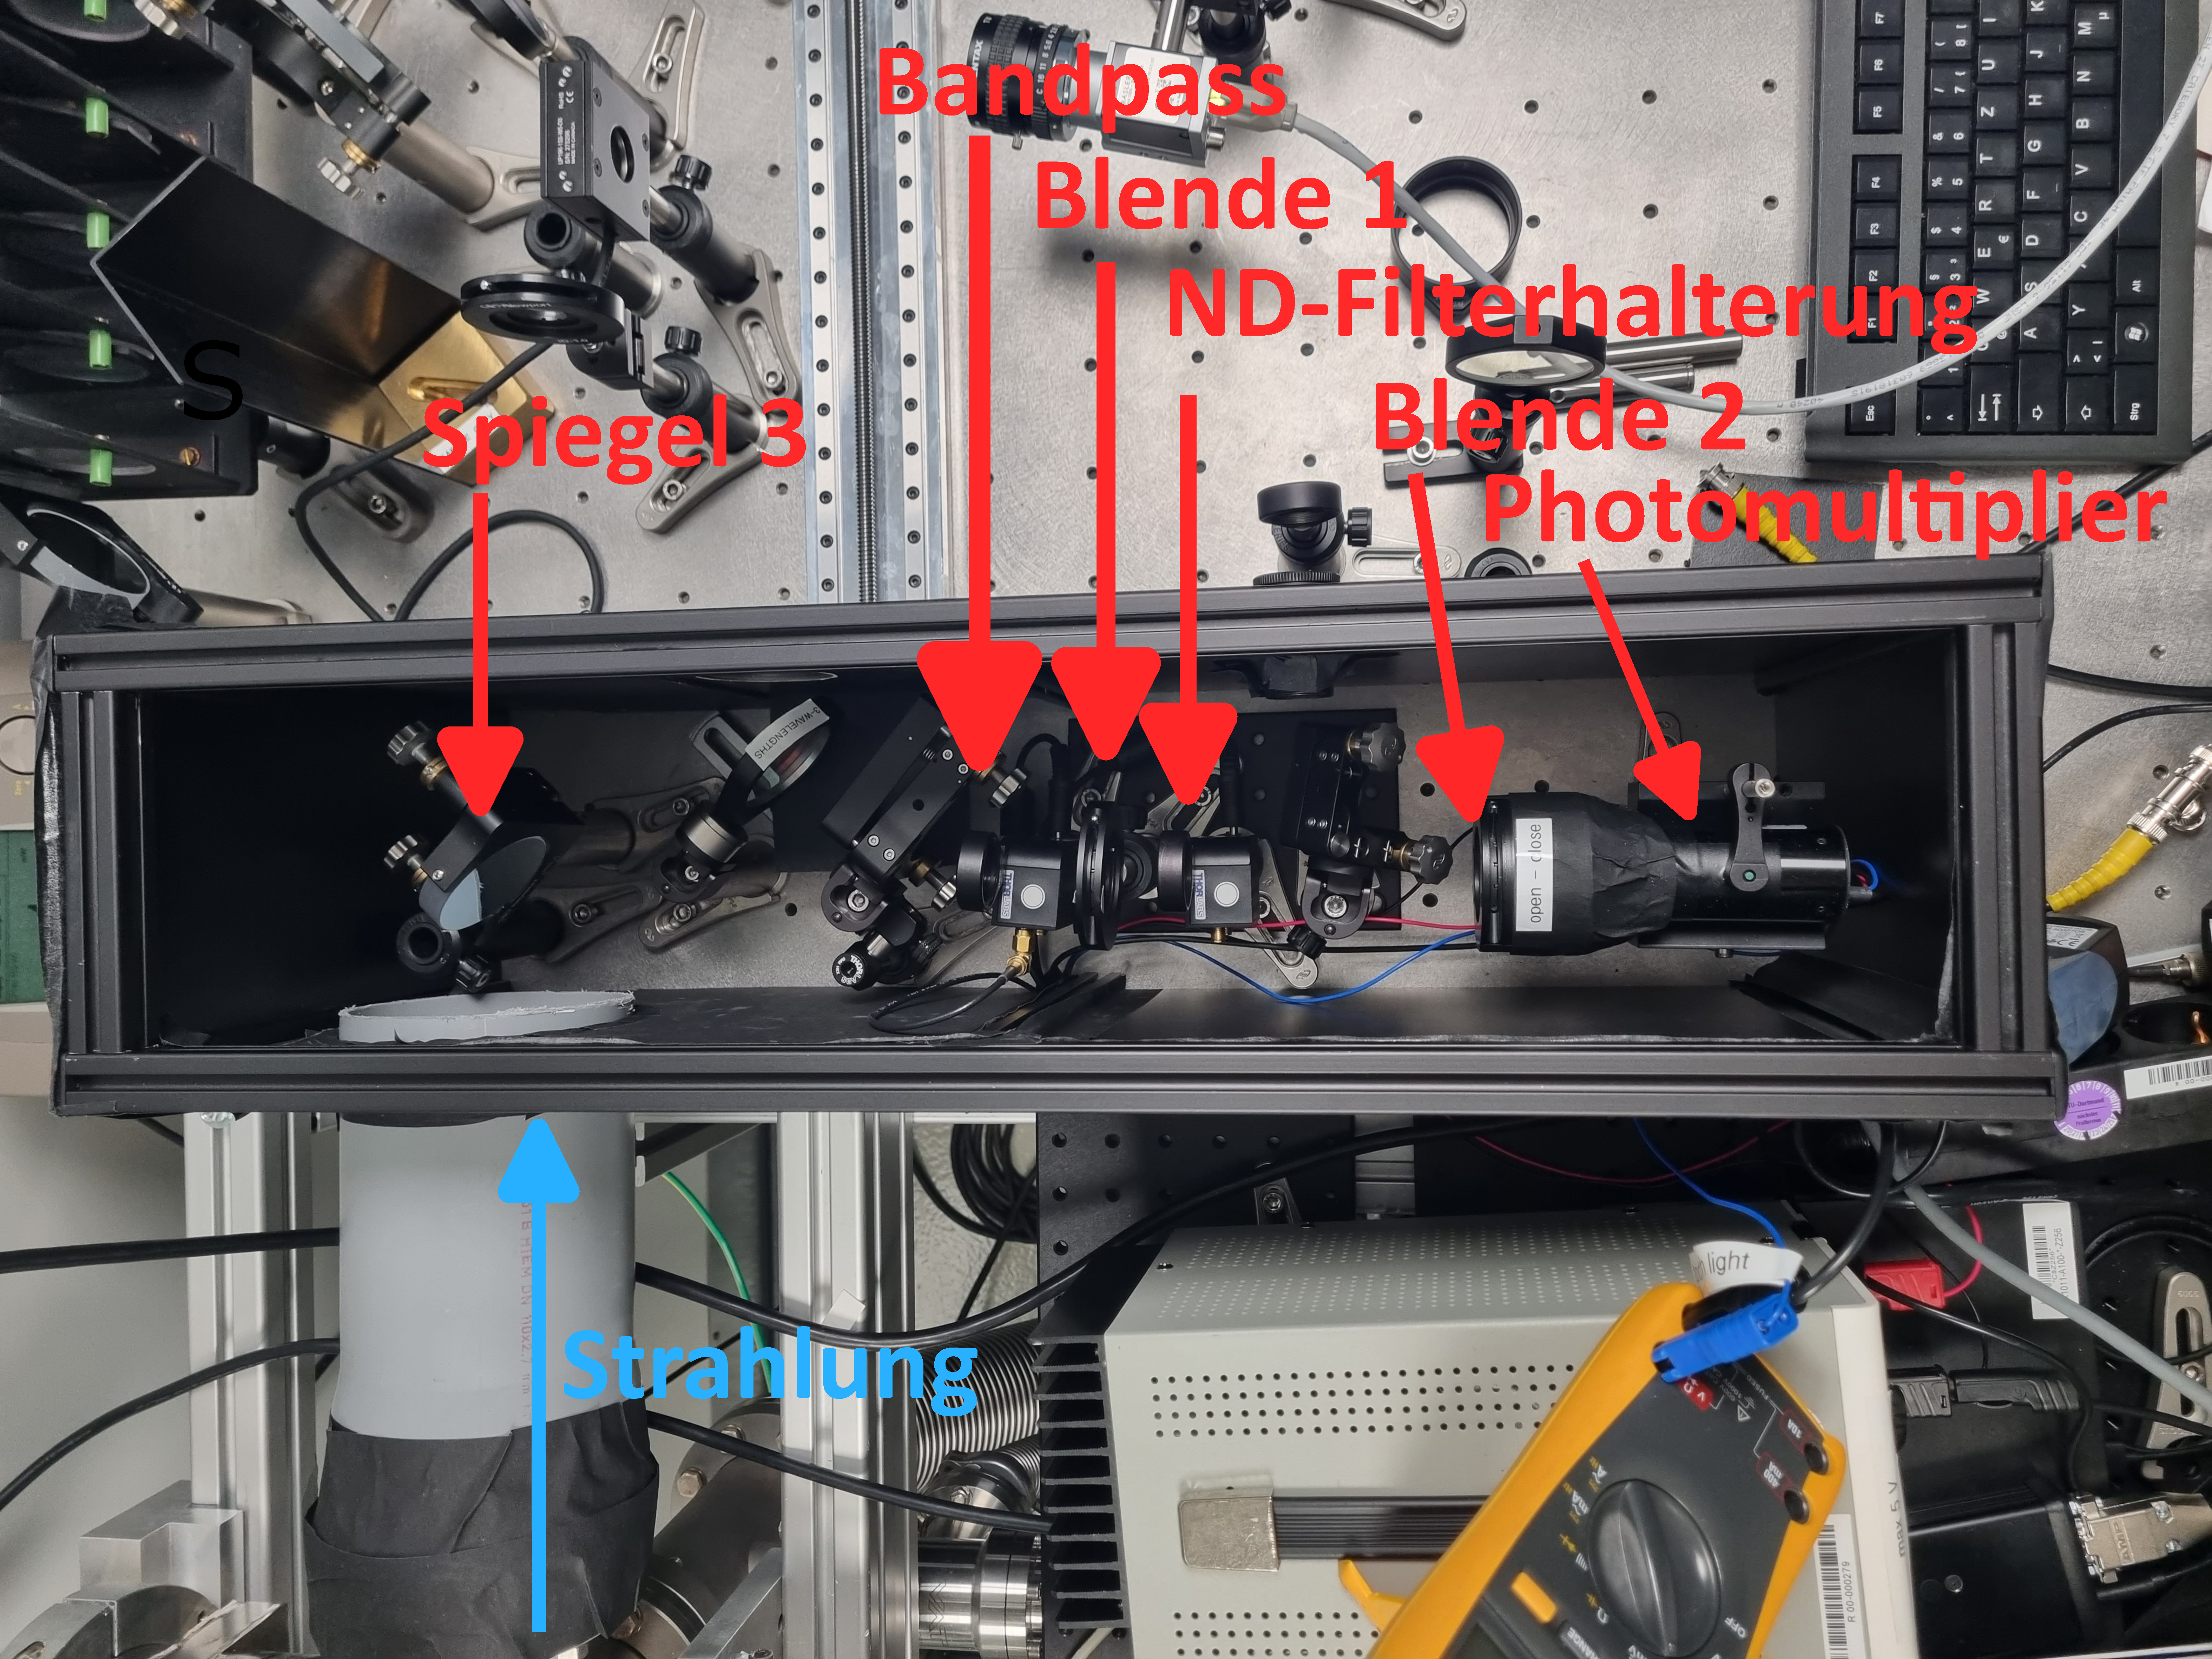
\includegraphics[width=16cm, height=12cm]{content/bilder/blackbox.pdf}
  \caption{Zu sehen ist der optische Aufbau. Nachdem die Strahlung in das Labor gespiegelt wurde wird sie durch
    eine Blende, einen Bandpass und einem ND-Filter abgeschwächt bevor sie auf den Photomultiplier trifft. }
  \label{fig:blackbox}
\end{figure}


\subsection{Der Photomultiplier}
\label{sec:Photomultiplier}
Für alle Experimente wurde der selbe Photomultiplier verwendet. Es handelt sich um einen Hamamatsu
H11870. Er arbeitet mit einer Spannung von lediglich fünf Volt und ist daher leicht zu handhaben.
Für jedes detektirte Photon gibt er einen Puls von etwa $\SI{9}{\nano\second}$ länge bei circa 
$\SI{2,2}{\volt}$ aus.



\subsection{Oszilloskop}
\label{sec:Oszilloskop}
Für die mit dem Oszilloskop durcheführten Messungen wurde ein LeCroy waveSurfer 104MXs-A mit einer 
Abtastrate von $\SI{5}[symbol]{\giga\sample\per\second}$verwendet. 

\subsection{TDC7200}
\label{sec:TDC}
Beim TDC7200 handelt es sich um einen Time to Digital Converter. Dieser besitzt einen Eingang für ein 
Start Signal und einen Eingang für ein Stop Signal. Der Chip misst die Zeit zwischen den steigenden oder 
fallenden Flanken der Signale. Die gemessenen Zeiten können dann über einen SPI Bus ausgelesen werden.
Das geschieht in diesem Aufbau durch einen Raspberry Pi. Dieses Verfahren funktioniert in nahezu Echtzeit. 
Daher kann mit diesem Aufbau leicht eine Füllstruktur errechnet und über das EPICS Protokoll im Netzwerk 
zur verfügung gestellt werden. Als Startsignal wird der DELTA Umlauftrigger genutzt. Als Stopsignal wird 
das Signal des Photomultipliers genutzt. 


\begin{figure}
  \centering
  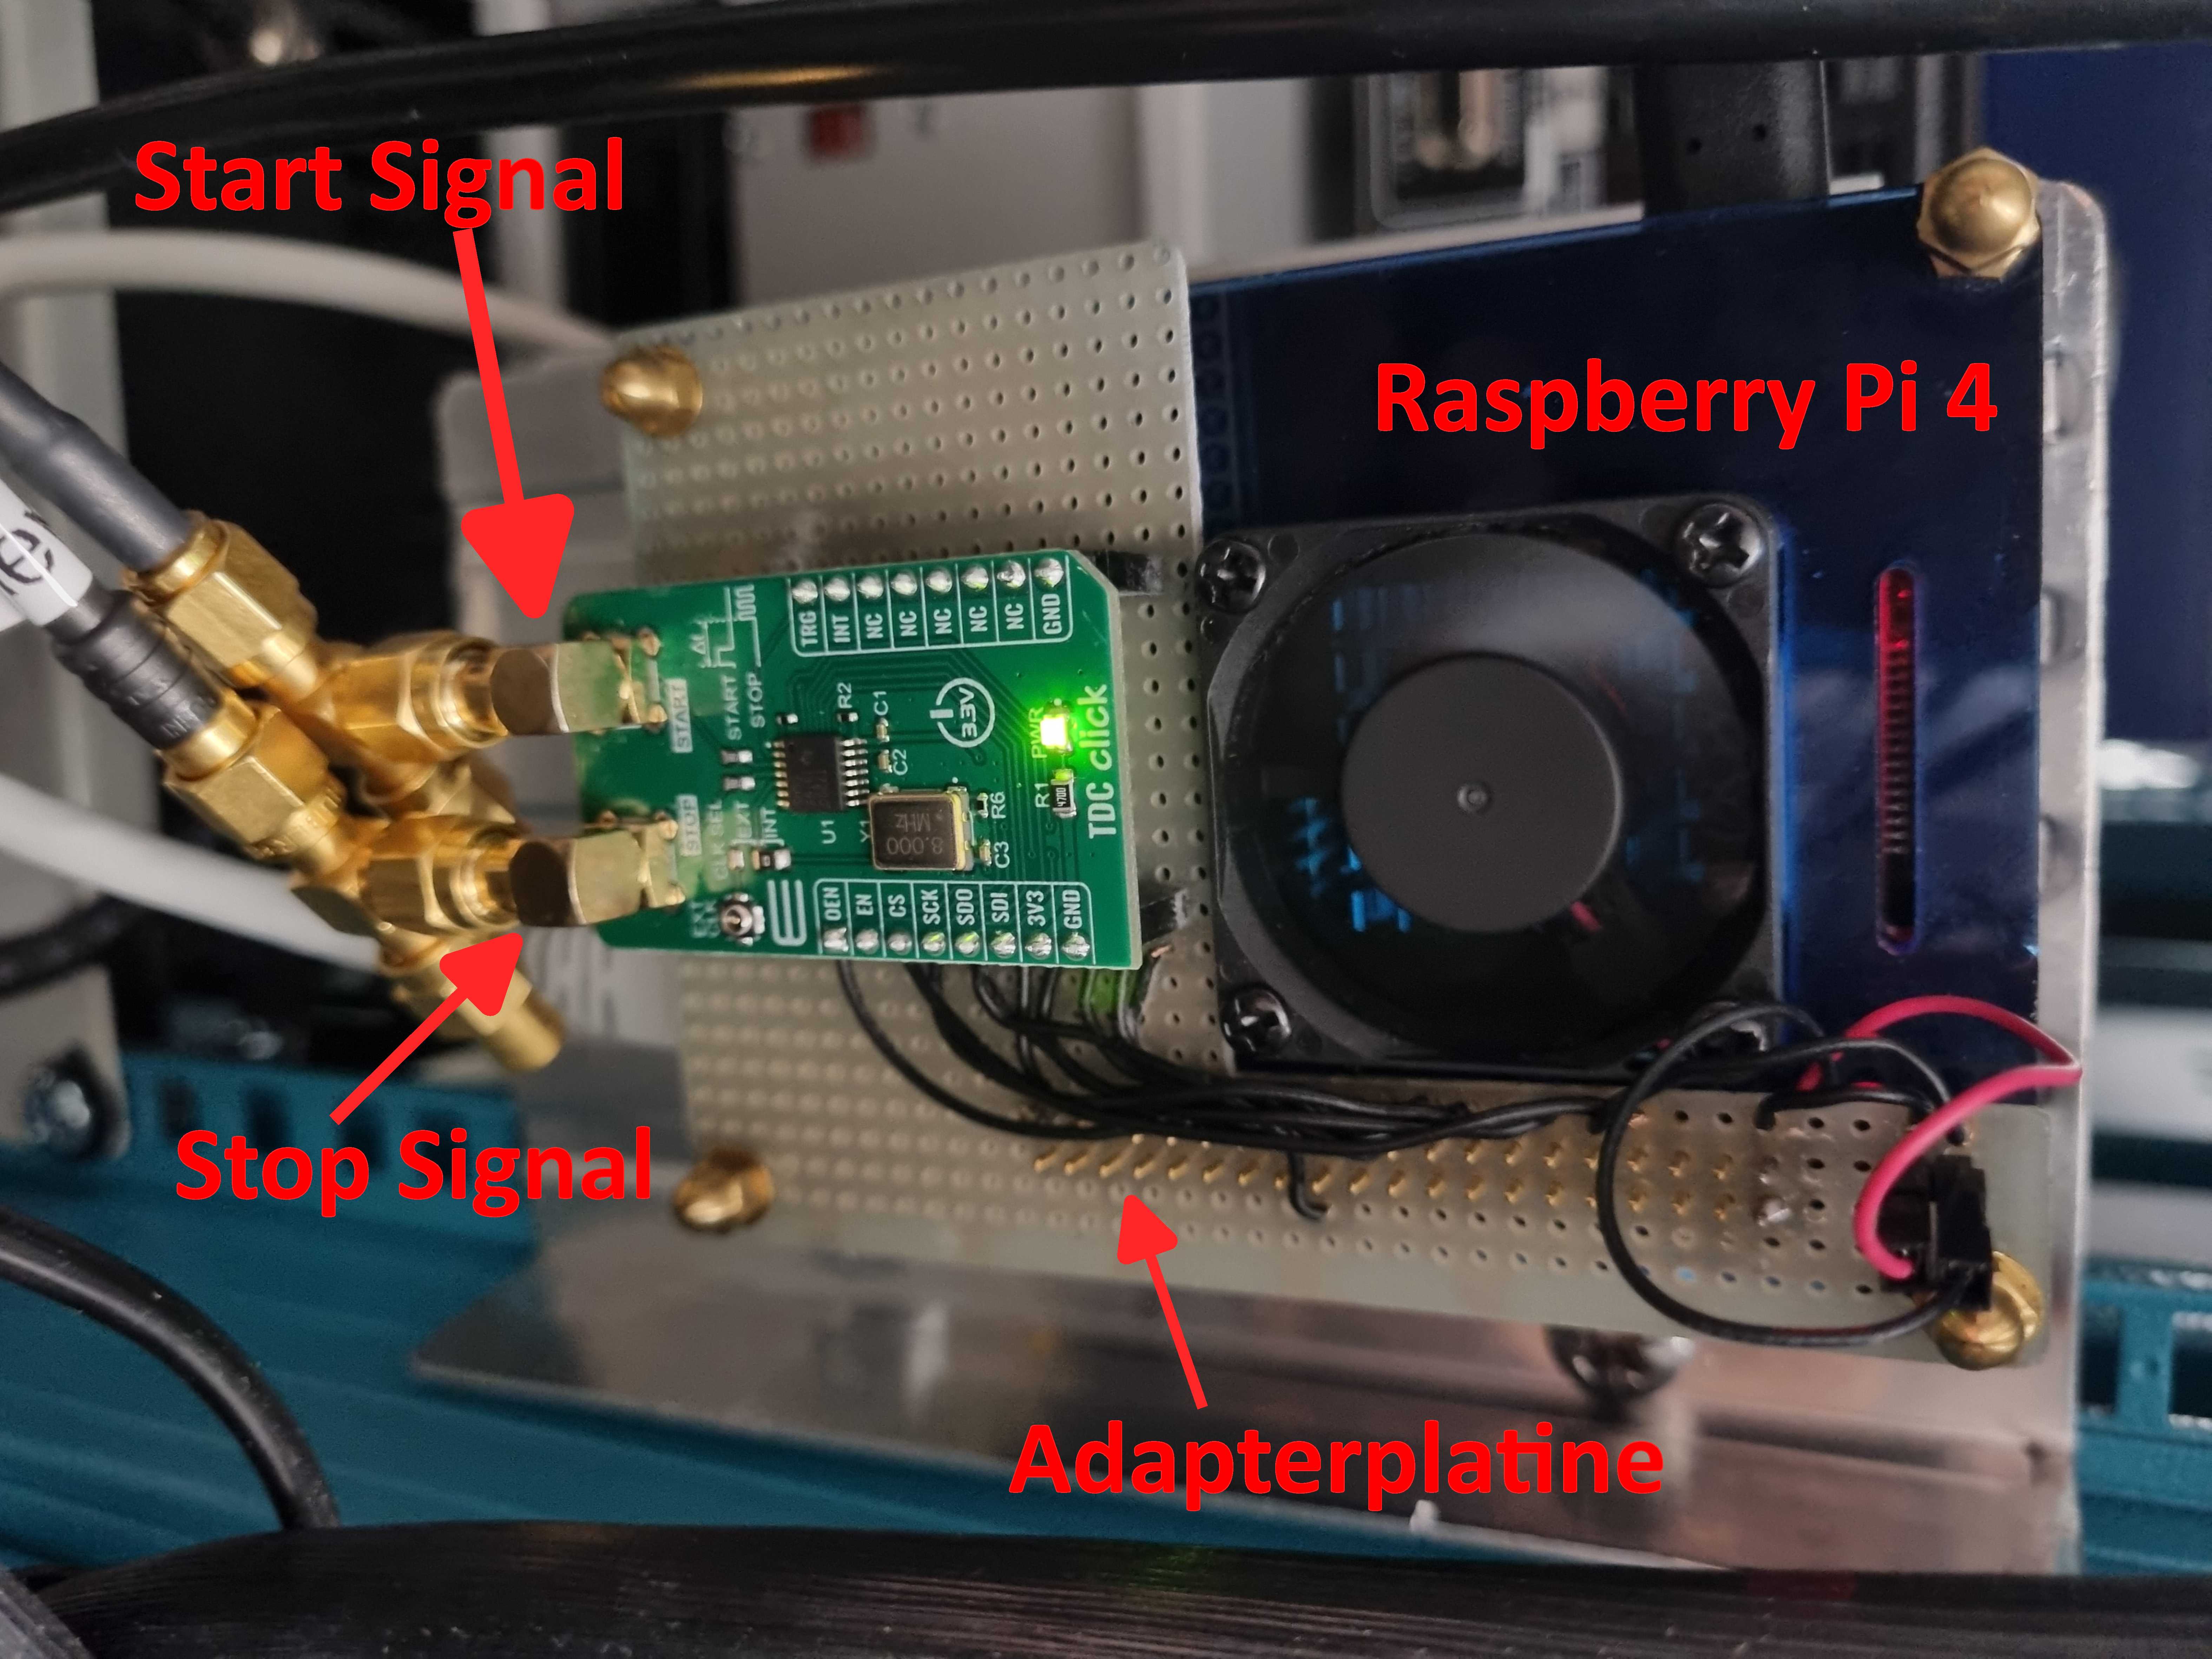
\includegraphics[width=16cm, height=12cm]{content/bilder/raspi.pdf}
  \caption{Auf dem Raspberry Pi befindset sich eine handgelöttete Adapterplatine welche fest mit dem Gehäuse
    des Raspberry Pis verschraupt ist und dessen GPIOs mit den Pins der Platine verbindet auf welcher der TDC7201
    aufgelötet ist. Start- und Stopsignal werden über koaxialkabel mit SMA Verbindern geliefert. Diese werden noch
    kurz vor dem Bord über ein T-Stück auf $\SI{50}{\ohm}$ abgeschlossen, da das TDC Board an sich eher einen offenen
    Abschluss darstellt.}
  \label{fig:raspi}
\end{figure}

\begin{figure}
  \centering
  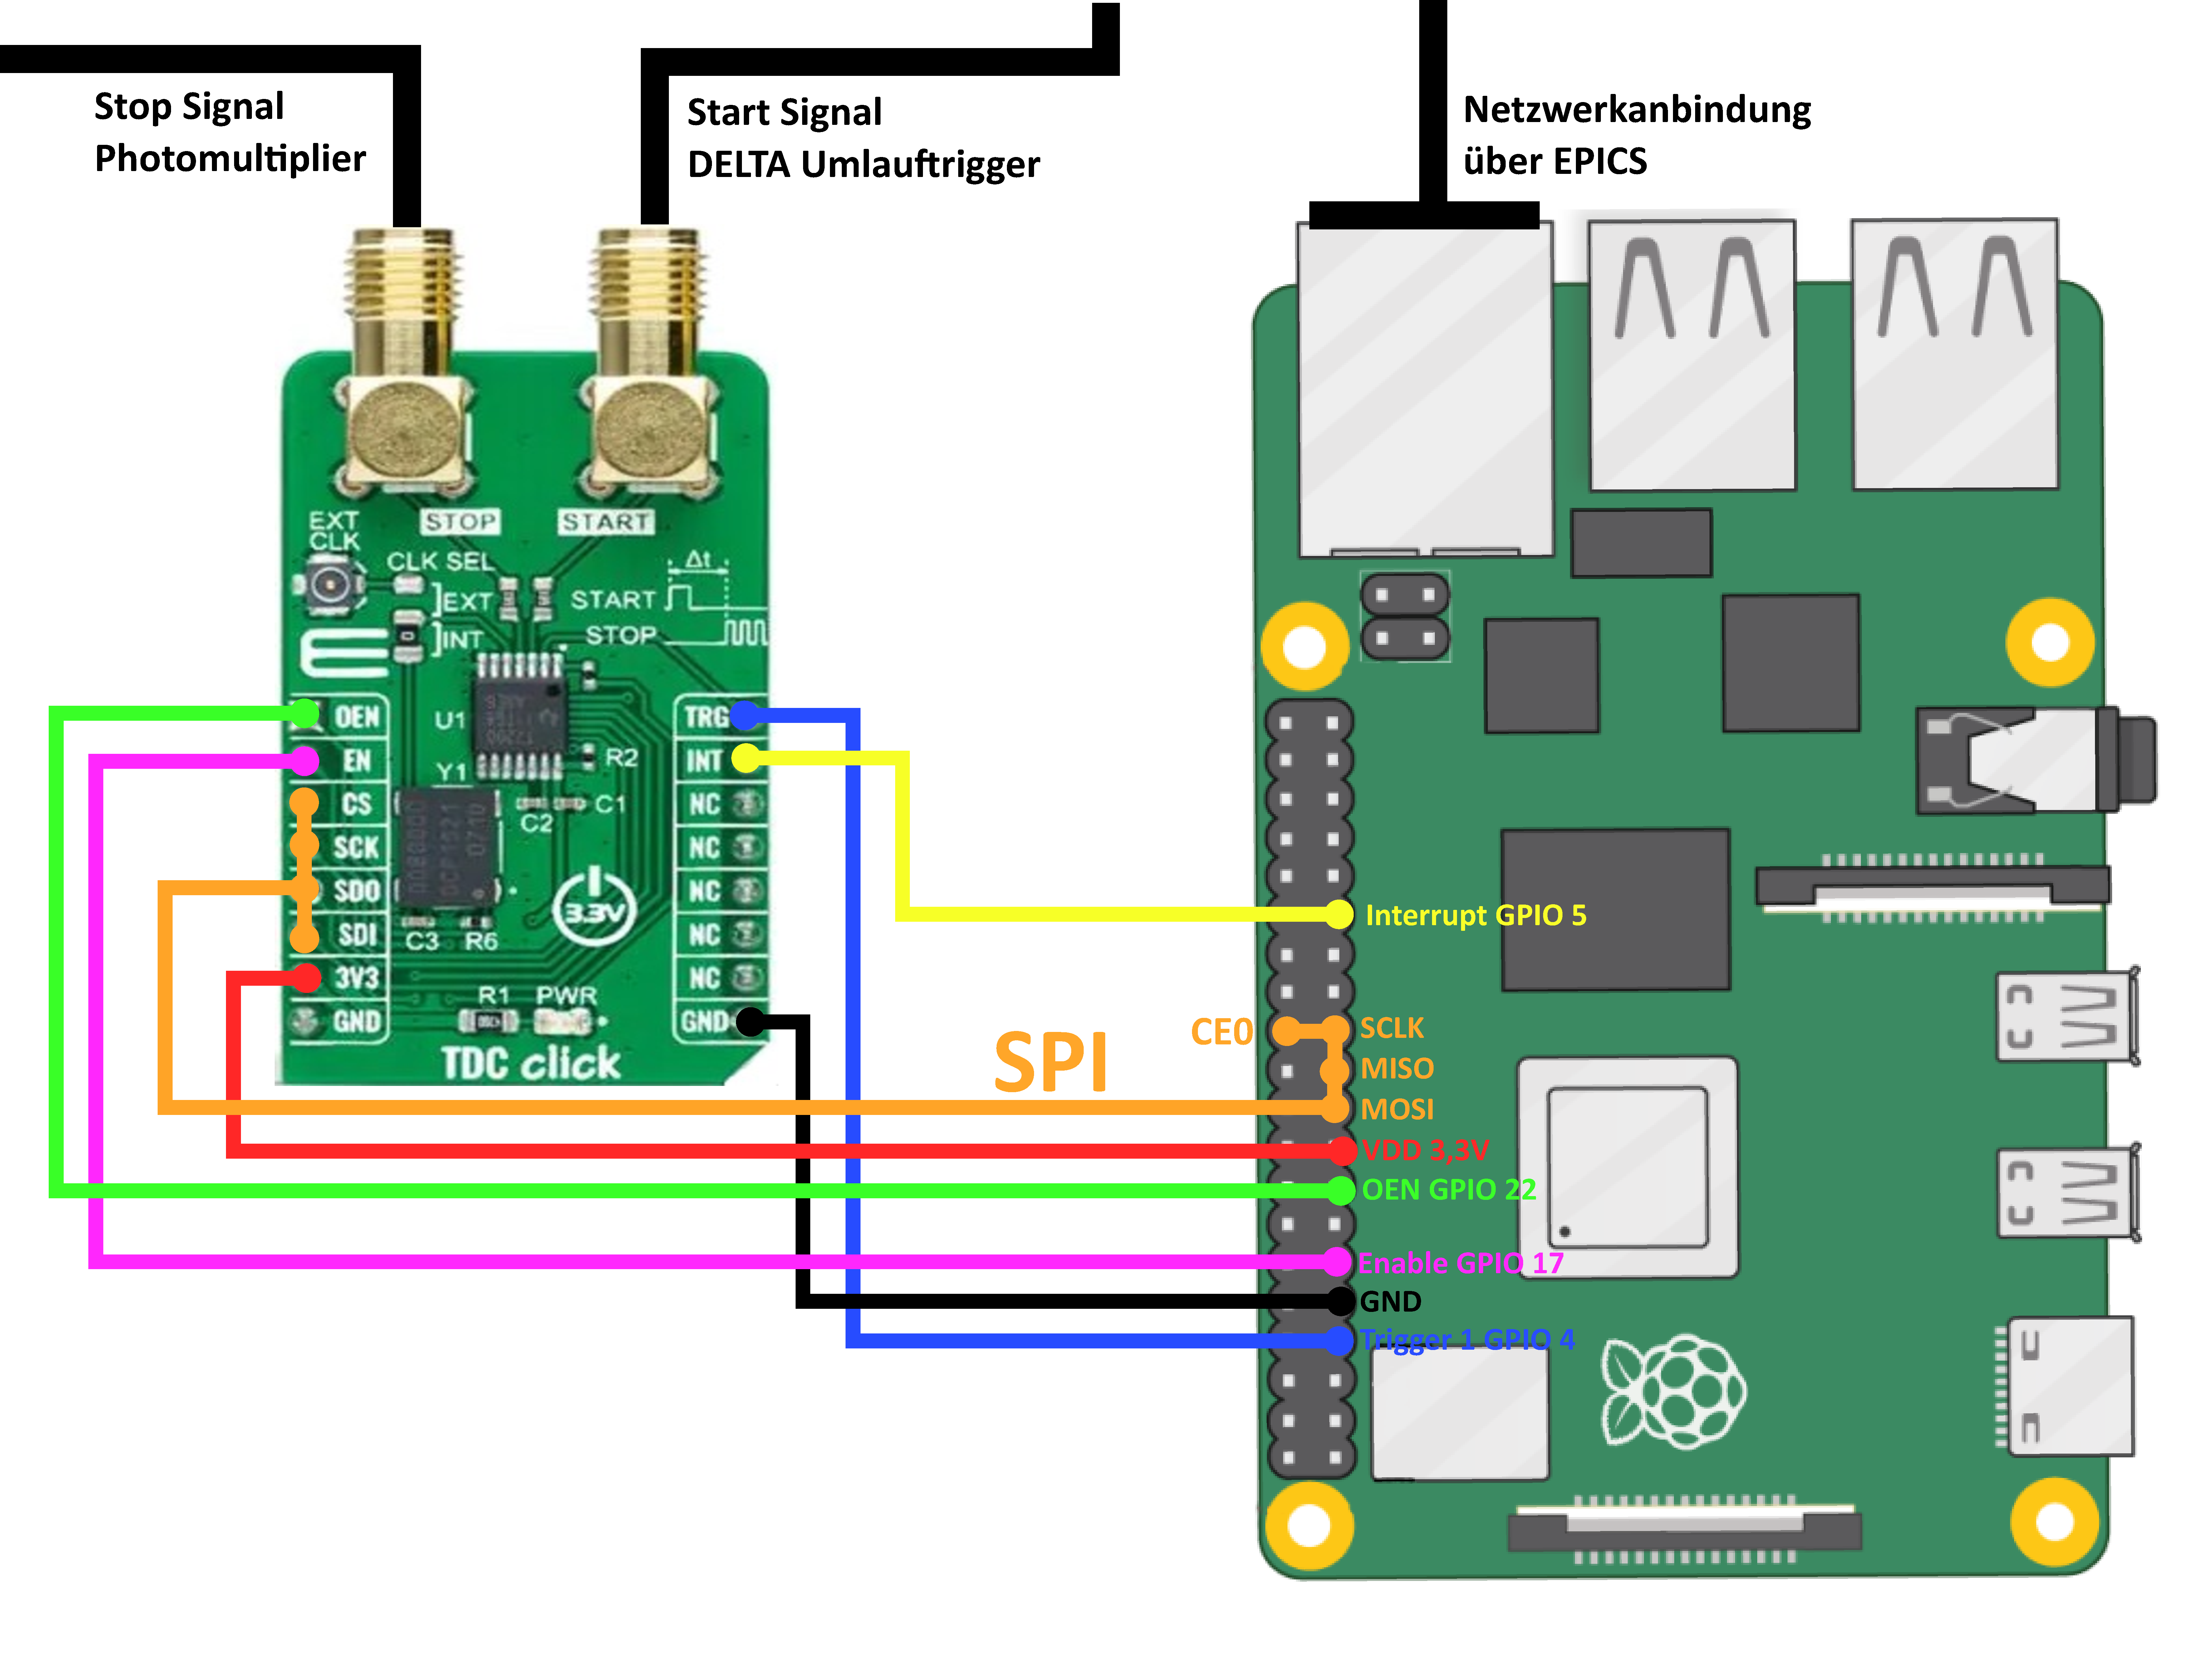
\includegraphics[width=16cm, height=12cm]{content/bilder/RaspiTdcSchaltung.pdf}
  \caption{Der Raspberry Pi ist über den SPI Bus (GPIO 10 MOSI, GPIO 9 MISO, GPIO 8 CE0 und GPIO 11 SCLK) mit dem TDC Board verbunden. 
    Zudem liefert der Raspberry Pi die benötigte Betriebsspannung von $V_{DD}=\SI{3,3}{\volt}$. Außerdem ist an GPIO 4 der
    Trigger-, an GPIO 17 der Enable-, an GPIO 22 der OEN und an GPIO 5 der Interrupteingang des TDC Boards angeschlossen. } 
  \label{fig:raspitdcschaltung}
\end{figure}


\begin{figure}
  \centering
  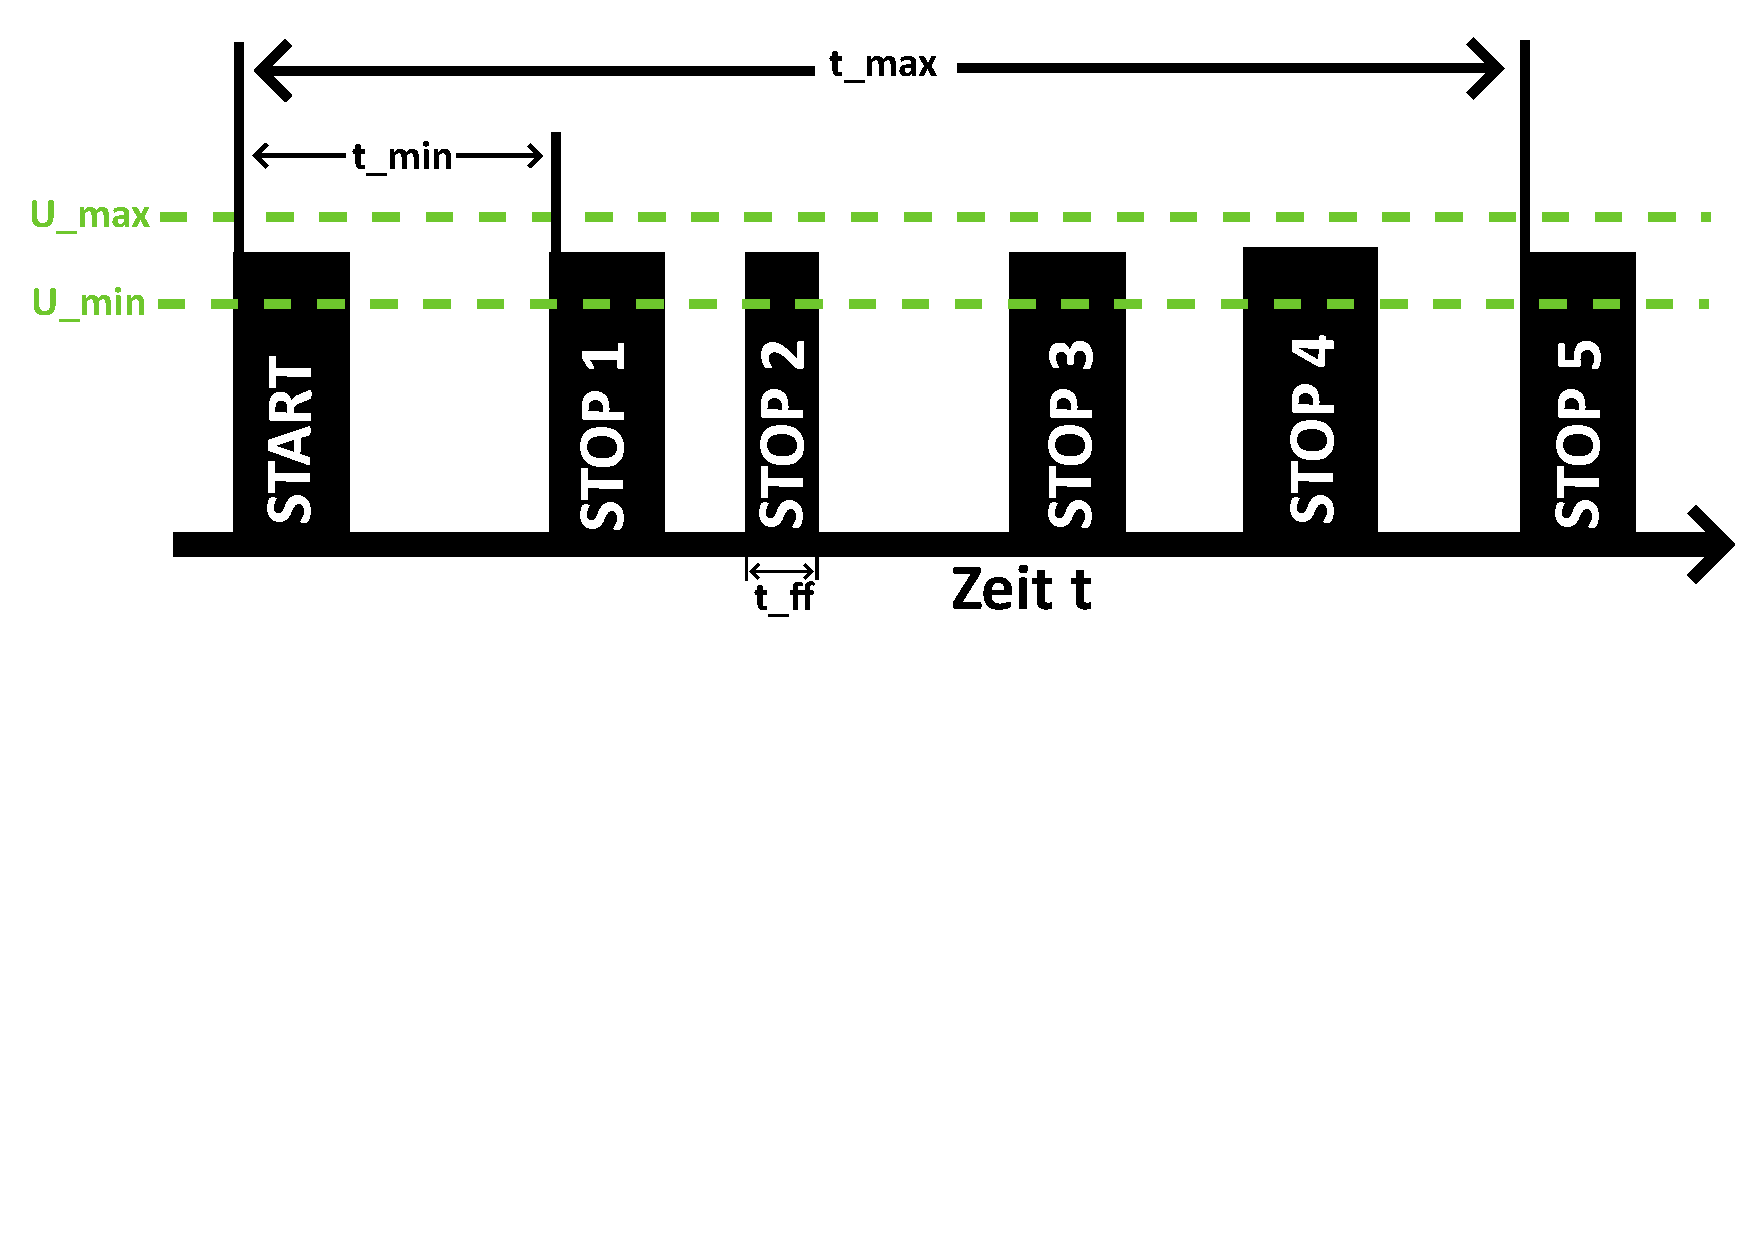
\includegraphics[width=16cm, height=12cm]{content/bilder/ZeitstrukturTDC.pdf}
  \caption{Der TDC7200 ist in der Lage bis zu fünf Stopsignale zu bearbeiten und kann dabei je nach 
    Einstellung entweder auf die steigende oder auf die fallende Flank des jeweiligen Start- oder
    Stopsignals reagieren. In den gemachten Experimenten wurde stehts die steigende Flanke genutzt. Die
    Spannung der Signale muss mindestens $U_{min}=0,7\times V_{DD}=\SI{2,31}{\volt}$ und darf maximal 
    $\SI{3,6}{\volt}$ betragen. } 
  \label{fig:zeitstrukturTDC}
\end{figure}

\subsection{Time Tagger}
\label{sec:TimeTagger}
Der Time Tagger ist ein dem in \autoref{sec:TDC} beschriebenen Aufbau ähnliches kommerzielles Produkt
der Firma Swabian Instruments.
\section{Durchführung}
\label{sec:Durchfuehrung}

\subsection{Auflösung des TDC bestimmen}
\label{sec:AufloesungTDC}

\subsection{Probleme bei der Messung mittels TDC}
\label{sec:ProblemeTDC}

\subsubsection{Geschwindigkeit des Delaygenerators}
\label{sec:Delaygenerator}

\subsubsection{Geschwindigkeit des TDC}
\label{sec:GeschwindigkeitTDC}

\subsection{Messungen mit dem Oszilloskop}
\label{sec:MessungenOszilloskop}

\subsection{Messungen mit dem Time Tagger}
\label{sec:MessungenTT}

\section{Auswertung}
\label{sec:Auswertung}
\section{Diskussion}
\label{sec:Diskussion}


\printbibliography{}

\section*{Anhang}
\label{sec:Anhang}
Programmcode



\end{document}
